% This version of CVPR template is provided by Ming-Ming Cheng.
% Please leave an issue if you found a bug:
% https://github.com/MCG-NKU/CVPR_Template.

\documentclass[review]{cvpr}
%\documentclass[final]{cvpr}

\usepackage{times}
\usepackage{epsfig}
\usepackage{graphicx}
\usepackage{amsmath}
\usepackage{amssymb}
\usepackage{caption}
\usepackage{subcaption}
\usepackage{gensymb}
\usepackage{stackrel}
\newcommand{\X}{\mathbf{X}}
\newcommand{\R}{\mathbf{R}}
\newcommand{\D}{\mathcal{D}}
\newcommand{\dtmax}{\Delta \theta_\text{max}}

% Include other packages here, before hyperref.

% If you comment hyperref and then uncomment it, you should delete
% egpaper.aux before re-running latex.  (Or just hit 'q' on the first latex
% run, let it finish, and you should be clear).
\usepackage[pagebackref=true,breaklinks=true,colorlinks,bookmarks=false]{hyperref}

\def\cvprPaperID{****} % *** Enter the CVPR Paper ID here
\def\confYear{CVPR 2021}
%\setcounter{page}{4321} % For final version only

\begin{document}

%%%%%%%%% TITLE
\title{Exploiting and Refining Probabilistic Depth Estimates with RGB and Triangulating Light Curtain Fusion}

\author{Yaadhav Raaj ~ Siddharth Ancha ~ Joe Bartels ~ Robert Tamburo ~ Srinivasa G. Narasimhan\\
Carnegie Mellon University\\
{\tt\small \{ryaadhav, sancha, bartels, rtamburo, srinivas\}@cs.cmu.edu}
% For a paper whose authors are all at the same institution,
% omit the following lines up until the closing ``}''.
% Additional authors and addresses can be added with ``\and'',
% just like the second author.
% To save space, use either the email address or home page, not both
}

\maketitle

%%%%%%%%% ABSTRACT
\begin{abstract}
Programmable Triangulating Light Curtains are a low-cost, high speed and high resolution approach to depth sensing, but require the user to specify a 2.5D ruled surface over where sensing should occur. Objects that intersect this surface show up with a high intensity, while those that don't do not. We have devised a novel algorithm, that exploits prior depth distributions from either Monocular or Stereo RGB cameras to sample depth in regions of the world most uncertain using the Light Curtain. We then incorporate this data to get a refined depth estimate over time. We evaluate this setup with real world real-time experiments such as in the context of Advanced driver-assistance systems (ADAS)
\end{abstract}

\iffalse
Introduction
Prior Work
   Joe's Paper
   Sid's Paper
   other stuff
Sensor setup
   Light Curtain Basics
   Our Jeep setup
   Calibration process (eqs. here)
Adaptive Sensing Formulation (say Light Curtain Only)
   Simulator
   3D Tensor to store Depth (initialization)
   Ray 2D Projection into Flat Plane
   Planning Formulation/Strategies Default/M1
   Probabilistic Formulation (Inverted Gaussian Model)
   Experiments (show Sim vs Real world, Indoor vs Outdoor):
      Basic Sweep visualization (sanity check)
      Prior sweeping approach
      Non Inverted vs Inverted
      STD encoding the uncertaintiy etc.
      Default vs M1 (and diff strategies)
   Having a Prior Depth (what if we had)
   Experiments here
         Show convergence speed/accuracy etc.
Generating Prior from RGB
   NN Formulation figure
   Soft CE, QPower, Left/Right Consistency (RGB + Depth), Smoothness
   Experiments:
      Show table for above
   LC Integration
   Experiments:
      Effect/Speedup of having a Prior
      
      3D Upsampling of Lidar
      Time feedback vs no
      Deep Learning vs no Deep Learning (Ruled Surface etc.)
Outdoor Experiments:
   etc.
Future Work
\fi


%%%%%%%%% BODY TEXT
\section{Introduction}

Programmable Triangulating Light Curtains were introduced last year, and have demonstrated viability in being a low cost (1k\$ vs lidar's ~25k\$), high spatial angular resolution (0.02$\degree$ vs lidar's  0.4$\degree$), and high frame-rate (~60fps vs lidar's ~20fps) sensor. They have demonstrated having strong returns in the presence of artifacts such as smoke, and also in seeing small targets such as pedestrians further away. They do however, require a user to specify at what depth per pixel one want's sensed, through providing a physically possible 2.5D ruled surface that intersects the world to provide returns. 

Conversely, depth estimation through RGB cameras have been a heavily researched area, but do not provide the realiability in estimates as compared to a Lidar, which can be cost prohibitive. This has made both RGB and Lidar's en-masse adoption in safety critical systems such as Advanced driver-assistance systems (ADAS) rare. 

Our work, looks into marrying both modalities to counter each sensor's limitations, through the use of Geometric, Probabilistic and Physical constraints. We begin by formulating an iterative Bayesian inference approach to depth sensing using the Light Curtain alone, leveraging on Depth Probability Volume (DPV) and corresponding 2D Uncertainty Field (UF) representations. We then build upon existing planning framework based on Dynamic Programming using the Light Curtain's Galvanometer velocity and acceleration constraints. Lastly, we expand upon the state of the art in Generating and Exploiting Probabilistic Depth Estimates using Deep Learning based approaches, and use that as a prior to drive Light Curtain placement.

\section{Prior Work}

Lorem ipsum dolor sit amet, consectetur adipiscing elit, sed do eiusmod tempor incididunt ut labore et dolore magna aliqua. Ut enim ad minim veniam, quis nostrud exercitation ullamco laboris nisi ut aliquip ex ea commodo consequat. Duis aute irure dolor in reprehenderit in voluptate velit esse cillum dolore eu fugiat nulla pariatur. Excepteur sint occaecat cupidatat non proident, sunt in culpa qui officia deserunt mollit anim id est laborum. \cite{wang2018programmable} \cite{bartels2019Agile}

Lorem ipsum dolor sit amet, consectetur adipiscing elit, sed do eiusmod tempor incididunt ut labore et dolore magna aliqua. Ut enim ad minim veniam, quis nostrud exercitation ullamco laboris nisi ut aliquip ex ea commodo consequat. Duis aute irure dolor in reprehenderit in voluptate velit esse cillum dolore eu fugiat nulla pariatur. Excepteur sint occaecat cupidatat non proident, sunt in culpa qui officia deserunt mollit anim id est laborum. \cite{Ancha_2020_ECCV}

Lorem ipsum dolor sit amet, consectetur adipiscing elit, sed do eiusmod tempor incididunt ut labore et dolore magna aliqua. Ut enim ad minim veniam, quis nostrud exercitation ullamco laboris nisi ut aliquip ex ea commodo consequat. Duis aute irure dolor in reprehenderit in voluptate velit esse cillum dolore eu fugiat nulla pariatur. Excepteur sint occaecat cupidatat non proident, sunt in culpa qui officia deserunt mollit anim id est laborum.

Lorem ipsum dolor sit amet, consectetur adipiscing elit, sed do eiusmod tempor incididunt ut labore et dolore magna aliqua. Ut enim ad minim veniam, quis nostrud exercitation ullamco laboris nisi ut aliquip ex ea commodo consequat. Duis aute irure dolor in reprehenderit in voluptate velit esse cillum dolore eu fugiat nulla pariatur. Excepteur sint occaecat cupidatat non proident, sunt in culpa qui officia deserunt mollit anim id est laborum.

\section{Sensor Setup}

\subsection{Light Curtain Basics}

\begin{figure}[h]
   \centering
   \begin{minipage}{0.5\textwidth}
       \centering
       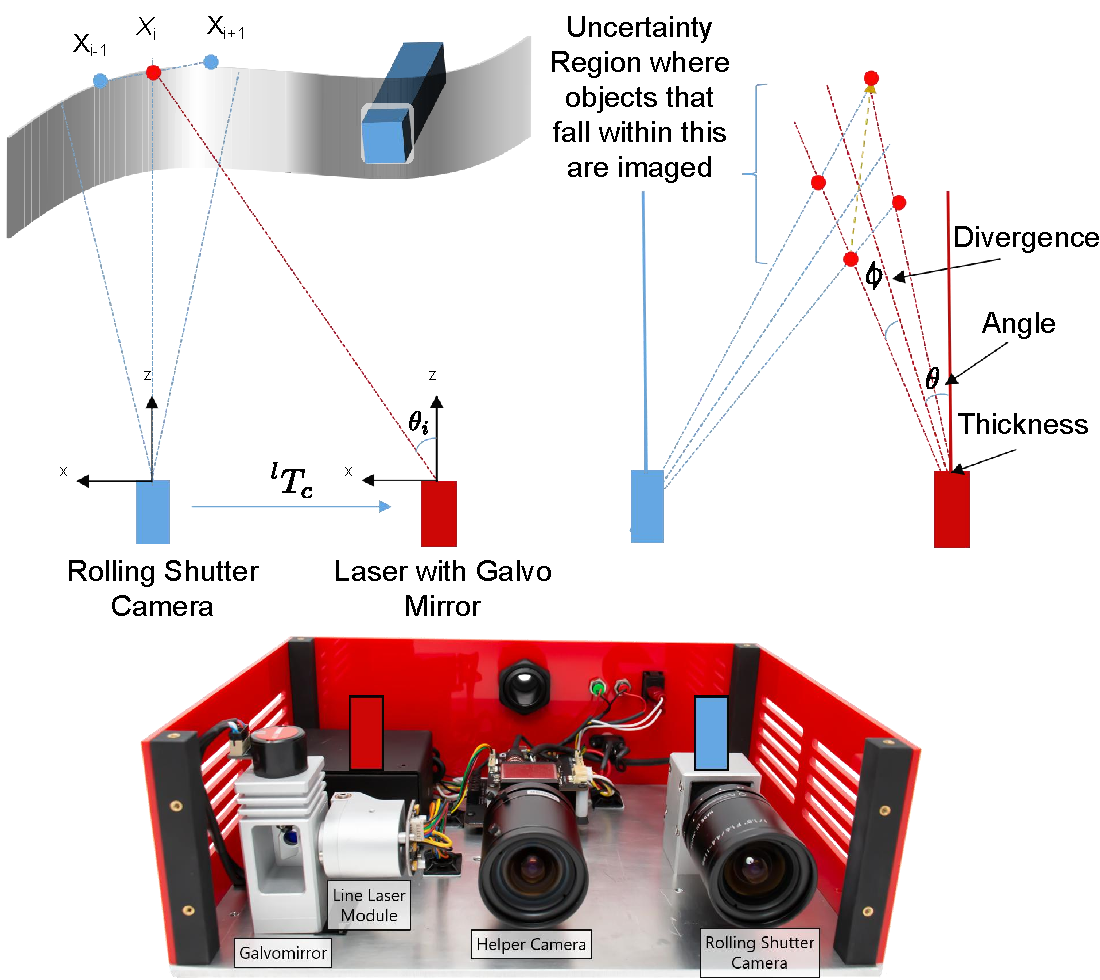
\includegraphics[width=1.0\textwidth]{figures/LC.pdf} % first figure itself
   \end{minipage}\hfill
   % \begin{minipage}{0.3\textwidth}
   %     \centering
   %     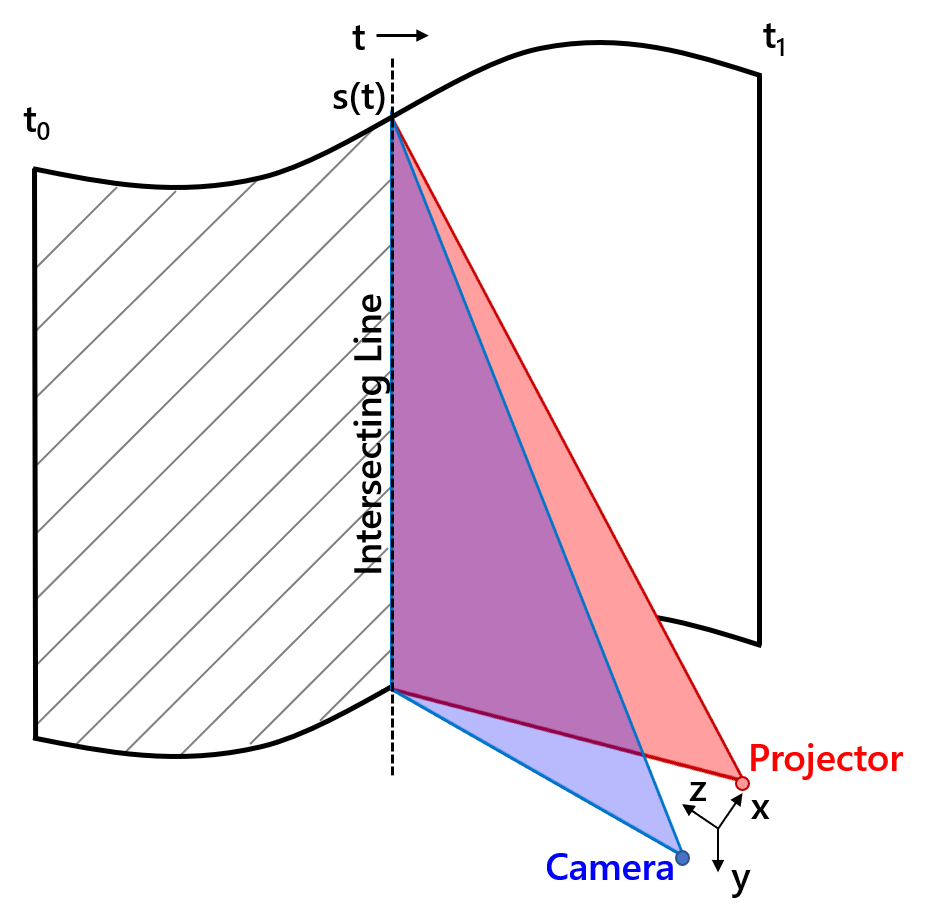
\includegraphics[width=0.9\textwidth]{light_curtain_iso.png} % second figure itself
   % \end{minipage}
   \centering
   \caption{The Programmable Light Curtain device \cite{bartels2019Agile}, consisting of a steerable laser, an IR camera and a microcontroller, capable of generating slices in space to image in 3D}
\end{figure}

The Light Curtain consists of a rolling shutter NIR camera flipped vertically, a Line Laser module and a Galvomirror. The rolling shutter NIR camera runs in sync with the laser, where each row of the camer can be thought of as a plane with some divergence going out vertically into space. The laser/projector fires a similar vertical sheet of light as a plane into space, which intersects with the camera's vertical plane to produce an intersecting volume. We call this the \textit{thickness} of the curtain. Any objects that lie within this space will then be imaged by the camera. We we will know the 3D position of said objects. Hence, a top-down XZ profile can be provided in the NIR camera's frame, to generate a ruled 3D curtain surface at ~50fps

\subsection{Simulator}

\begin{figure}[h]
   \centering
   \begin{minipage}{0.4\textwidth}
       \centering
       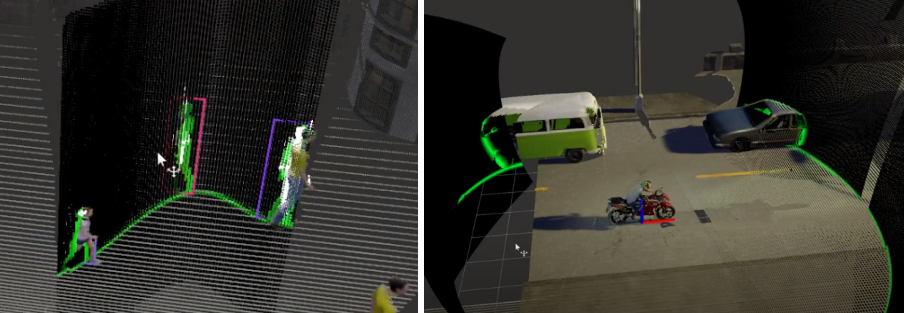
\includegraphics[width=1.0\textwidth]{figures/sim.png}
   \end{minipage}\hfill
   \centering
   \caption{Light Curtain Simulator in CARLA environment}
\end{figure}
\vspace{-.1in}
We also designed and open sourced a light curtain simulator to test and evaluate our algorithms, allowing for the Light Curtain paramters such as NIR instrinsics, Laser/NIR extrinsincs, Galvomirror speed etc. to be controlled.

\subsection{Sensor Array}

\begin{figure}[h]
   \centering
   \begin{minipage}{0.5\textwidth}
       \centering
       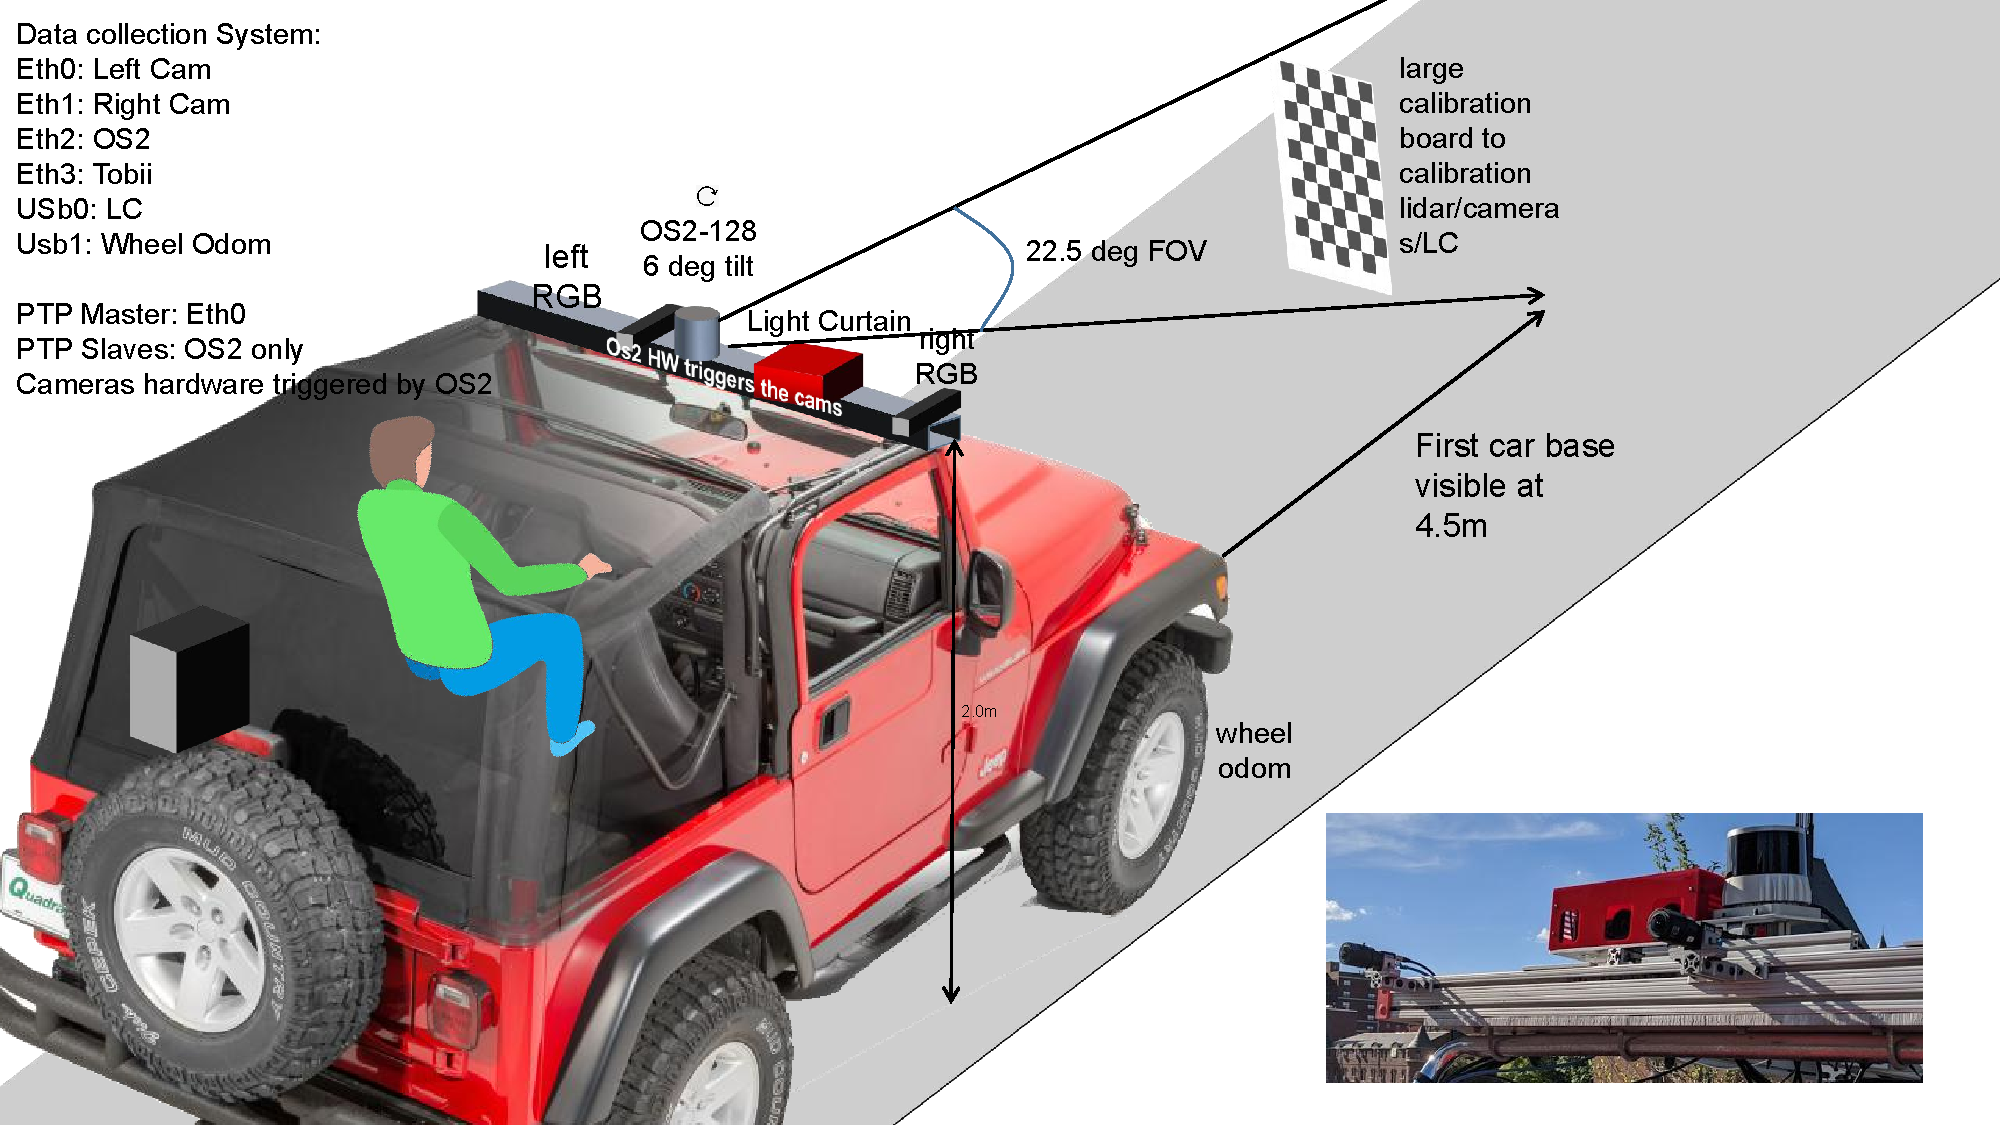
\includegraphics[width=1.0\textwidth]{figures/array.pdf}
   \end{minipage}\hfill
   \centering
   \caption{Sensor Array consisting of a Stereo camera pair, the Light Curtain device and a 128 Beam Lidar}
\end{figure}

Our sensor array consists of a Stereo Camera Pair with a baseline of 0.7m, the Light Curtain device located close to the main/left camera to minimize depth/volume transformation parallax artifacts, and an Ouster OS2-128 Lidar for algorithm accuracy validation and to assist in training depth estimation networks. All sensors are calibrated to the common reference frame of the left RGB camera.

\section{Formulation}

We begin by looking at a Light Curtain only problem of adaptively discovering the depth of a scene. We wouldn't know the path along the rays/pixels on which an object may lie/intersect, hence we choose to go with a sampling based approach. We treat each ray as initially having either a uniform distribution, or a gaussian with a large variance in the center, and we attempt to formulate our problem with a Recursive Bayesian update approach.

\subsection{Representation}

\smallskip
Our state space is represented as a tensor of some fixed resolution [320x240] with each pixel in image $I$ encoding the depth value $\mathbf{d}(u,v)$ as a bernoulli distribution $P(\mathbf{d}(u,v))$. $D_{c}$ represents the list of depths quantizing the space of each pixel defined within $(d_{min}, d_{max})$ of some fixed size $N$ [64], resulting in a Depth Probability Volume (DPV) tensor of size [64, 240, 320]
\begin{align}
   D_{c}=\left\{ d_{0}...d_{n}\right\} \quad d_{i}=d_{min}+(d_{max}-d_{min})*t 
   \label{eq:d_candi}
   \\
   P(\mathbf{d}(u,v))=I(u,v)
   \nonumber\\
   \sum_{d}\left(P(\mathbf{d}(u,v))\right)=1\qquad \mathbb{E}[P(\mathbf{d}(u,v))]=\mathbf{d}(u,v)
   \label{eq:depth_dist}
   %\vspace{-.1in}
\end{align}

While an ideal sensor could choose plan a path to sample in the full 3D volume, our Light Curtain device only has control over a collapsed XZ  space. Hence, we select a subset of rays that correspond to a plane that we wish to sample, and generate an Uncertainty Field (UF) as follows:
\begin{align}
   P(\mathbf{d}(u))=\frac{\sum_{u,v}P(\mathbf{d}{(u,v)}).\boldsymbol{1}}{\sum_{u,v}\boldsymbol{1}}
   \nonumber \\
   \;where\;h_{min}>\mathbb{E}[P(\mathbf{d}(u,v))]>h_{max}
   \label{eq:collapse}
   %\vspace{-.1in}
\end{align}

\begin{figure}[h]
   \centering
   \begin{minipage}{0.5\textwidth}
       \centering
       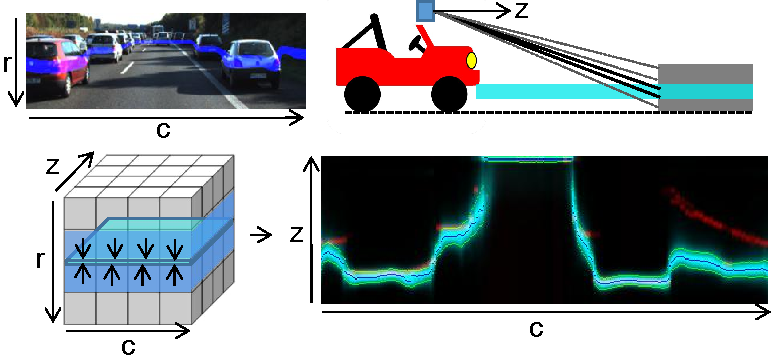
\includegraphics[width=1.0\textwidth]{figures/bev.pdf}
   \end{minipage}\hfill
   \centering
   \caption{Our state space consisting of a Depth Probability Volume (DPV) its corrsp Bird's Eye Uncertainty Field (UF)}
\end{figure}

\subsection{Curtain Planning}

With the Uncertainty Field (UF) extracted from the state space, we can use this to figure out where to place light curtains. We build upon prior work solving Light Curtain placement as a Constraint Optimization and Dynamic Programming problem. A single light curtain placement is defined by a set of $T$ control points $\{\X_t\}_{t=1}^T$. We wish to maximize the objective $J(\X_1, \dots, \X_T) = \sum_{t=1}^T UF(\X_t)$ where $UF(\X)$ is the uncertaintiy field probabilies at the anchor location of $\X$.

The control points $\{\X_t\}_{t=1}^T$, where each $\X_t$ lies on the the camera ray $\R_t$, must be chosen to satisfy the physical constraints of the light curtain device: $|\theta(\X_{t+1}) - \theta(\X_t)| \leq \Delta \theta_\text{max}$ with $\theta_\text{max}$ being the maximum angular velocity of the Galvomirror. The problem is also discretized such that $\X_{t} \in D_c\ $ and also lies along $\R_t$
\begin{align}
    &\arg \max_{\{\X_t\}_{t=1}^T} \sum_{t=1}^T UF(\X_t) \qquad \text{where}\ \X_t \in D_c\ \nonumber\\
    &\text{subject to}\ |\theta(\X_{t+1}) - \theta(\X_t)| \leq \dtmax,\ \forall 1 \leq t < T
    \label{eq:constraint}
\end{align}

\begin{figure}[h]
   \centering
   \begin{minipage}{0.5\textwidth}
       \centering
       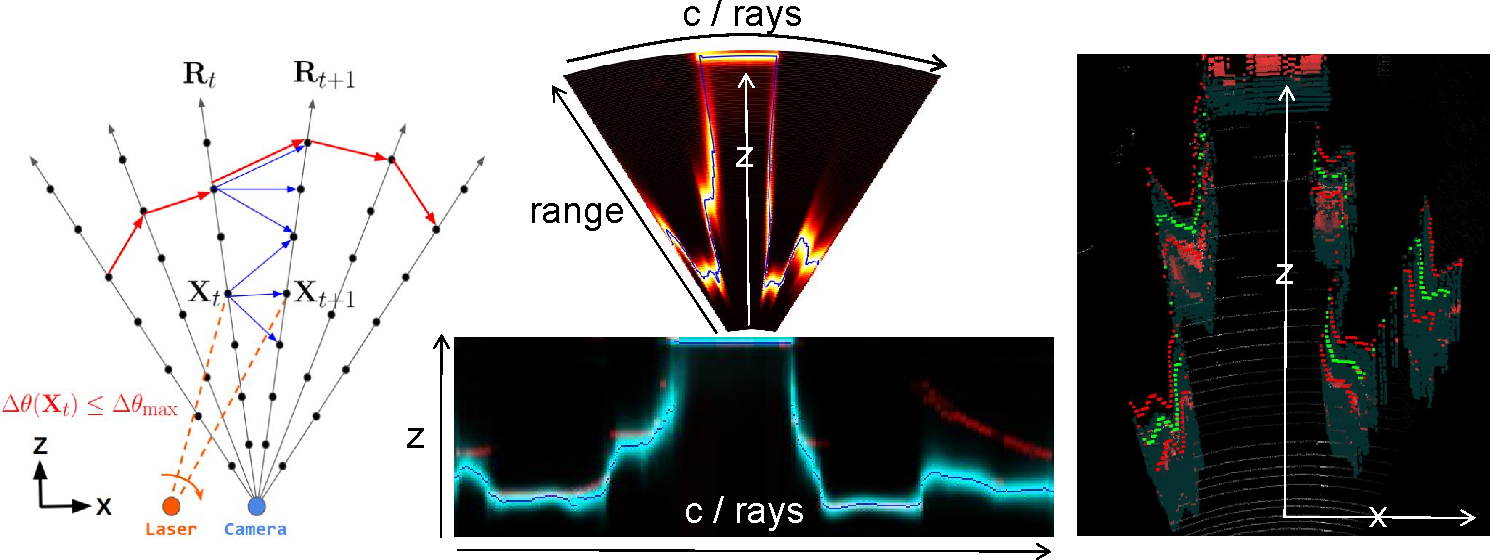
\includegraphics[width=1.0\textwidth]{figures/planner.pdf}
   \end{minipage}\hfill
   \centering
   \caption{Left: Light Curtain constraint graph subject to max angular velocity of Galvomirror. Right: Placing an optimal curtain along the highest probability region per column of rays}
\end{figure}

In the figure above, we have placed a single curtain along the highest probability region per column of rays, but ideally, we should place more curtains spanning the uncertaintiy of those distributions. To do this, we generate corresponding entropy fields $H(\X)_{i}$ to be fed to the planner from $UF(\X)$ based on two approaches: $m0$ attempts to normalize each ray's distribution $P(\mathbf{d}(u))$ and warp the distribution such that a selected span from the mean is maximized. $m1$ attempts to sample a point on the ray given $P(\mathbf{d}(u))$. 

\begin{figure}[h]
   \centering
   \begin{minipage}{0.5\textwidth}
       \centering
       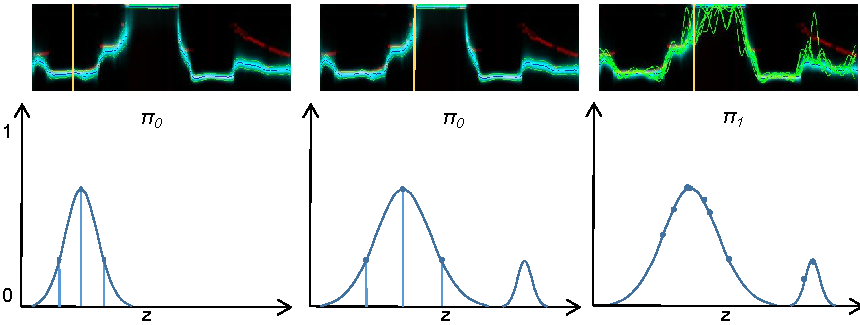
\includegraphics[width=1.0\textwidth]{figures/fields.pdf}
   \end{minipage}\hfill
   \centering
   \caption{We look at a depth distribution of one of the rays in UF (yellow line), and figure out where additional curtains (blue points) can be placed such as to maximize information gained. Observe that $m1$ is able to handle multimodal distributions}
   \label{fig:m0m1}
\end{figure}

As seen in Fig. ~\ref{fig:m0m1}, strategy $m0$ is able to generate fields that adaptively place additional curtains around a consistent span around the mean, but is unable to do so in cases of multimodal distributions. $m1$ on the other hand is able to place a curtain around the 2nd modality, albeit with a lower probability. The inconsistency from ray to ray in $m1$ however, may be impossible to image due to it exceeding the acceleration bounds, hence a spline fit is used with control points every 5 to 10 rays, resulting in an imagable but non-flat curtain placement. We see the effects of both in later experiments.

\subsection{Observation Model}

We now have returns from curtains $\mathbf{C}$ with each $\mathbf{C}_{i}$ containing $[x,y,z,i]$, the 3D position and intensity value in the same spatial resolution as $I$, planned based on a particular policy, conditioned on our prior distribution $P(\mathbf{d}_{t})$ at time $t$. We need to convert $\mathbf{C}_{i}$ into a likelihood distribution $P(\mathbf{c}_{t}|\mathbf{d}_{t})$, such that this Hidden Markov Model representation and sum of log likelihoods holds true:
\small
\begin{align}
   P\left(\mathbf{d}_{0},...,\mathbf{d}_{T},\mathbf{c}_{1},...,\mathbf{c}_{T}\right)= 
   P\left(\mathbf{d}_{0}\right)\mathbf{\mathbf{\prod}_{\mathrm{t=1}}^{\mathrm{T}}}P\left(\mathbf{c}_{t}|\mathbf{d}_{t}\right)P\left(\mathbf{d}_{t}|\mathbf{d}_{t-1}\right) \nonumber\\
   \log\left(P\left(\mathbf{c}_{t}|\mathbf{d}_{t}\right)\right)=\stackrel[i=0]{n}{\sum}\left(\log\left(P\left(\mathbf{c_{\mathit{i}}}_{t}|\mathbf{d}_{t}\right)\right)\right)
   \label{eq:hmm}
\end{align}
\normalsize

We represent $P\left(\mathbf{c_{\mathit{i}}}_{t}|\mathbf{d}_{t}\right)$ as a linear combination of a gaussian and a uniform distribution, where $\sigma$ is a function of the thickness of the light curtain as described earlier where $t\in[-1..1]$. $t$ is a function of the intensity value $i$, based on two possible profiles where $z$ either takes a value of 0.5 or 1.0, and $m$ is some control factor we tune:

\small
\begin{align}
   P\left(\mathbf{c_{\mathit{i}}}_{t}|\mathbf{d}_{t}\right)=\frac{\mathcal{N}\left(D_{c},\mu_{c},\sigma_{c}\right)\left(t\right)+U\left(D_{c}\right)(1-t)}{\sum\left(\mathcal{N}\left(D_{c},\mu_{c},\sigma_{c}\right)\left(t\right)+U\left(D_{c}\right)(1-t)\right)} \\
   t=\left(\frac{-1}{\left(z\right)+\left(mi\right)}\right)+1
   \label{eq:dist}
\end{align}
\normalsize

\begin{figure}[h]
   \centering
   \begin{minipage}{0.5\textwidth}
       \centering
       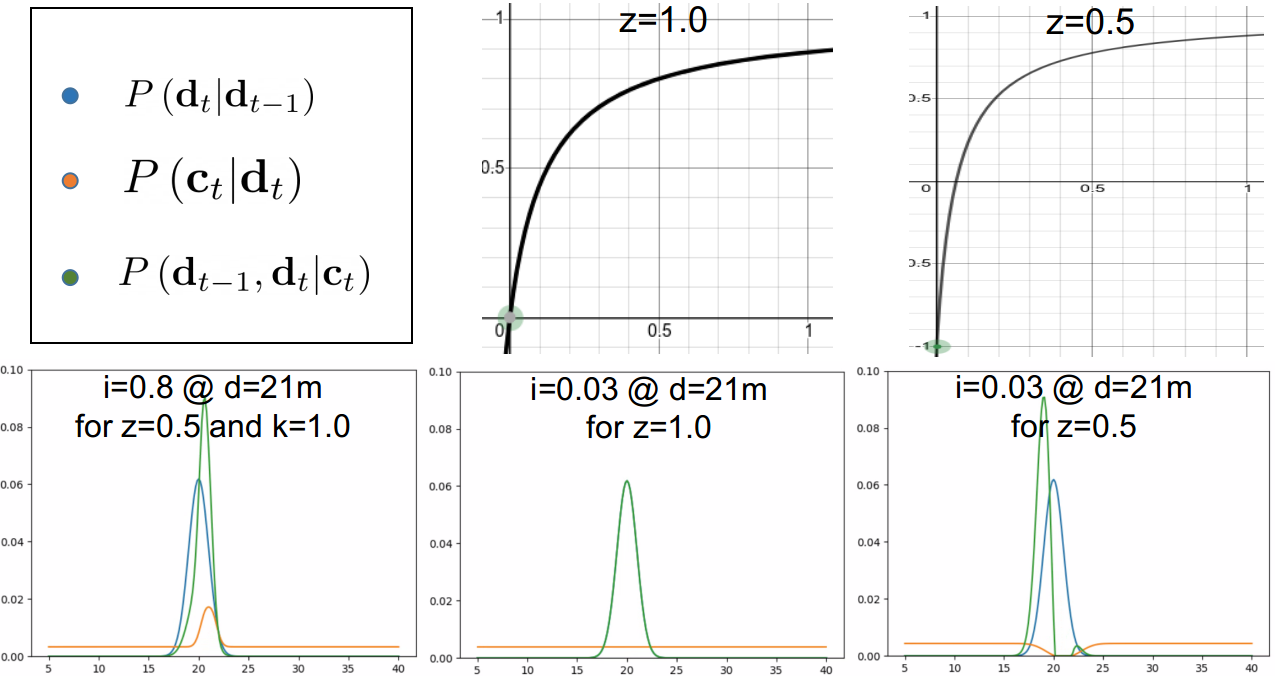
\includegraphics[width=1.0\textwidth]{figures/graphs.png}
   \end{minipage}\hfill
   \centering
   \caption{The effect on the posterior when getting a close to 0 intensity return from the Light Curtain when $z$ is either 1.0 or 0.5}
   \label{fig:updatemodel}
\end{figure}

As seen in Fig. ~\ref{fig:updatemodel}, as the intensity of the light curtain varies from 0 to 1 on the $x$ axis, we vary the value of $t$ on the $y$ axis. When $z$ is 0.5, low intensity returns (eg. < 0.1) results in a negative $t$ value. This means that when the intensity is high, a higher return results in a larger peak probability for both cases when $z$ is 1.0 or 0.5. But when the intensity is low or close to 0, $z=1.0$ causes $P\left(\mathbf{c}_{t}|\mathbf{d}_{t}\right)$ to tend to a uniform distribution, but $z=0.5$ to tend to an inverted gaussian. With this case, the rationale is that having no return at a location doesn't mean that we have derived no information at all, but rather, we know that this particular location is less likely to have an object and the rest of the the locations along the ray are equally uncertain/uniform. We show in experiments that this results in significantly faster convergence.

\section{Light Curtain only Experiments}

In this initial baseline, we attempt to track the Uncertainty Field (UF) depth error by computing the RMSE error metric $\sqrt{\stackrel[i=1]{n}{\sum}\frac{\left(\mathbb{E}\left(UF\left(u,q\right)\right)-\mathbf{d_{gt}}(u)_{i}\right)^{2}}{n}}$ against the ground truth. We use 3 scenarios: One in a KITTI driving scene using the LC simulator (a), one indoors in the basement using the both a simulated and real Light Curtain (b), and lastly in various outdoor driving scenes with the real device (c0/c1/c2). 

\begin{figure}[h]
   \centering
   \begin{minipage}{0.5\textwidth}
       \centering
       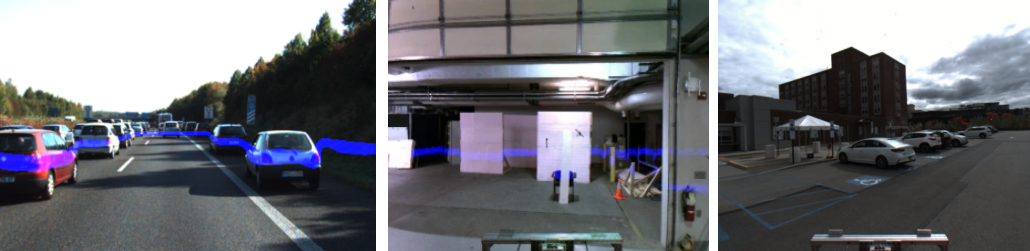
\includegraphics[width=1.0\textwidth]{figures/exp.png}
   \end{minipage}\hfill
   \centering
   \caption{Scenarios (a), (b), (c) from left to right}
   \label{fig:exp}
\end{figure}

\textbf{Planar Sweep:} A simple sanity check between simulation and the real sensor involves involves performing a uniform sweep across the scene in (b). 

\begin{figure}
   \centering
   \begin{minipage}{0.4\textwidth}
       \centering
       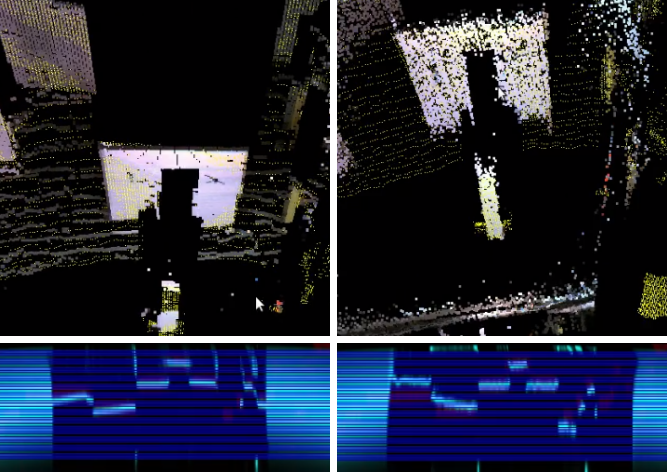
\includegraphics[width=1.0\textwidth]{figures/sweep.png}
   \end{minipage}\hfill
   \centering
   \caption{Doing a simple planar sweep across the scene. Colored pointcloud is the estimated depth, and Lidar ground truth in yellow. Left: LC simulated from the Lidar Depth. Right: Using the real LC}
   \label{fig:planarsweep}
\end{figure}

As seen in Fig. ~\ref{fig:planarsweep}, our simulated Light Curtain (LC) is able to reasonably match the real device. We also demonstrate how decreasing the steps the curtain takes reduces runtime but increases RMSE. Results seen in ~\ref{table:t1}

\noindent
\begin{table}[h]
   \centering
   \resizebox{0.9\linewidth}{!}{
   \begin{tabular}{|l|l|l|}
   \hline
    Policy&  Runtime/s&  RMSE/m\\ \hline
    Sweep 50 $\mathbf{C}$ Step 0.25m (Sim) &-  &1.156  \\ \hline
    Sweep 25 $\mathbf{C}$ Step 0.5m  (Sim) &-  &1.374  \\ \hline
    Sweep 50 $\mathbf{C}$ Step 0.25m (Real) &2  &1.284  \\ \hline
    Sweep 25 $\mathbf{C}$ Step 0.5m  (Real) &1  &1.574  \\ \hline
    Sweep 12 $\mathbf{C}$ Step 1.0m (Real) &0.5  &1.927  \\ \hline
   \end{tabular}}
   \caption{Error wrt to time and number of Sweep steps}
   \label{table:t1}
\end{table}

\textbf{Effect of Dynamic Sigma:} Earlier, we had noted how $\sigma(u,v,d_{u,v}^{c})$ defined for each $c_{k}$ measurement in $P\left(\mathbf{d}_{u,v}^{c_{k}}\right)$ is a function of the thickness of the curtain. We also experiment by making $\sigma(u,v,d_{u,v}^{c})$ fixed. We observe that it being a function of the curtain thickness is critical to better performance over larger steps/placements. Results in ~\ref{table:t2}

%\vspace{-.1in}
\noindent
\begin{table}[h]
   \centering
   \resizebox{0.9\linewidth}{!}{
   \begin{tabular}{|l|l|l|}
   \hline
    Policy&  Runtime/s&  RMSE/m\\ \hline
    Sweep $\mathbf{C}$ Step 0.25m (Dyn) &2  &1.276  \\ \hline
    Sweep $\mathbf{C}$ Step 0.5m  (Dyn) &1  &1.532  \\ \hline
    Sweep $\mathbf{C}$ Step 1.0m (Dyn) &0.5  &2.013  \\ \hline
    Sweep $\mathbf{C}$ Step 0.25m (Fixed) &2  &1.218  \\ \hline
    Sweep $\mathbf{C}$ Step 0.5m  (Fixed) &1  &1.658  \\ \hline
    Sweep $\mathbf{C}$ Step 1.0m (Fixed) &0.5  &2.290  \\ \hline
   \end{tabular}}
   \caption{$\sigma_{c}$ in generated $P\left(\mathbf{d}_{u,v}^{c_{k}}\right)$ being fixed vs being dynamic as a function of curtain thickness with real LC}
   \label{table:t2}
\end{table}

\textbf{Effect of Inverting Gaussian Model:} Our Observation Model ensures that the sensor distribution tends to an inverted gaussian when intensities are low. We test the effect on (a) and (b) in the above case, and in cases where low intensities tend to a uniform distribution. We see significantly improved performance when low intensities tend to an Inverted Gaussian rather than a uniform distribution. Results seen in ~\ref{fig:figure01} ~\ref{fig:invgau}

\begin{figure}[h]
    \centering
    \begin{minipage}{0.5\textwidth}
        \centering
        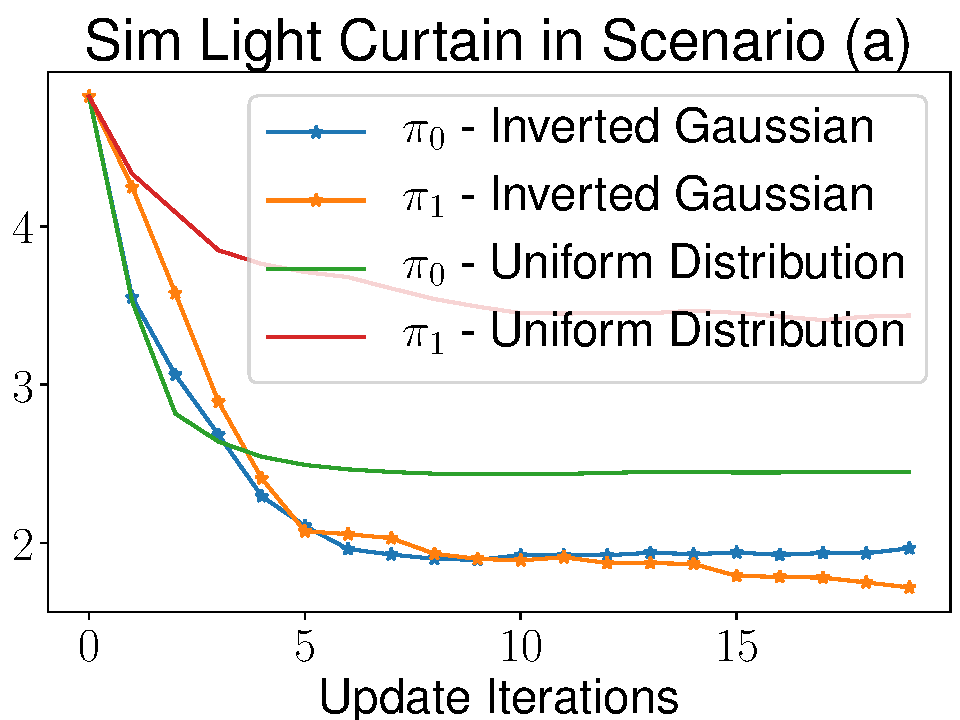
\includegraphics[width=0.49\textwidth]{figures/Figure_1.pdf}
        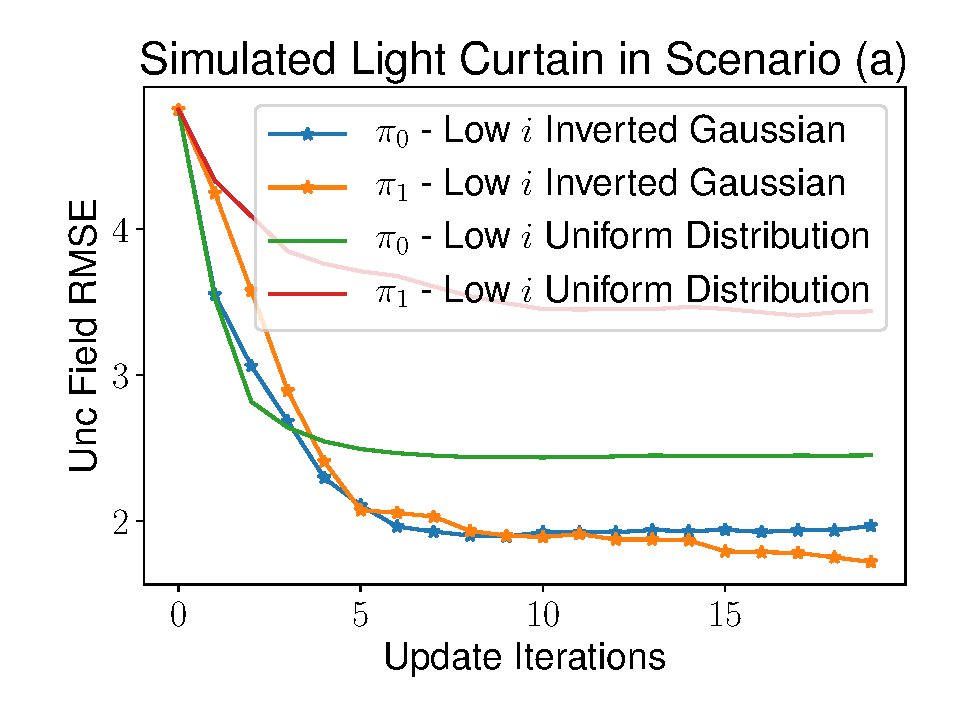
\includegraphics[width=0.49\textwidth]{figures/Figure_0.pdf}
    \end{minipage}\hfill
    \centering
    \caption{RMSE of Depth in UF over every iteration in scenarios left/(a) right/(b). Note the largely improved performance when low intensities tend to an Inverted Gaussian}
    \label{fig:figure01}
\end{figure}

 \begin{figure}[h]
    \centering
    \begin{minipage}{0.5\textwidth}
        \centering
        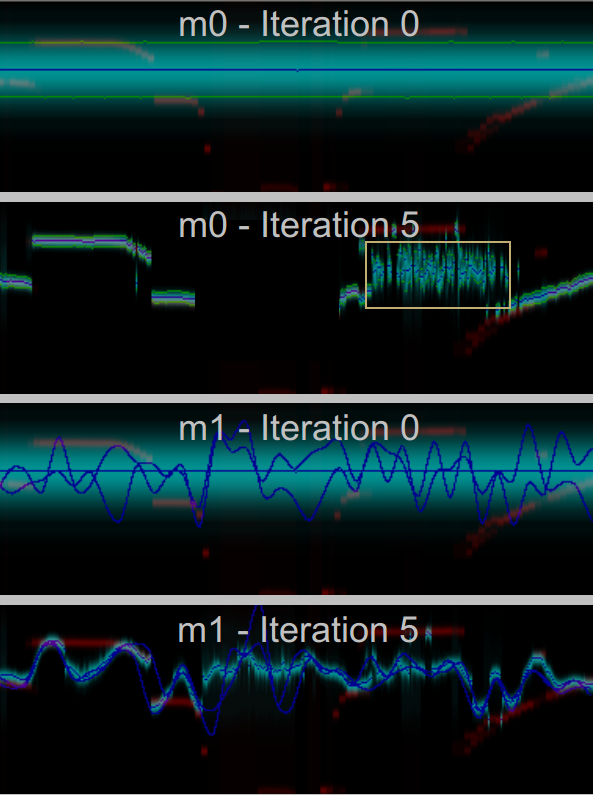
\includegraphics[width=0.49\textwidth]{figures/InvGau.png}
        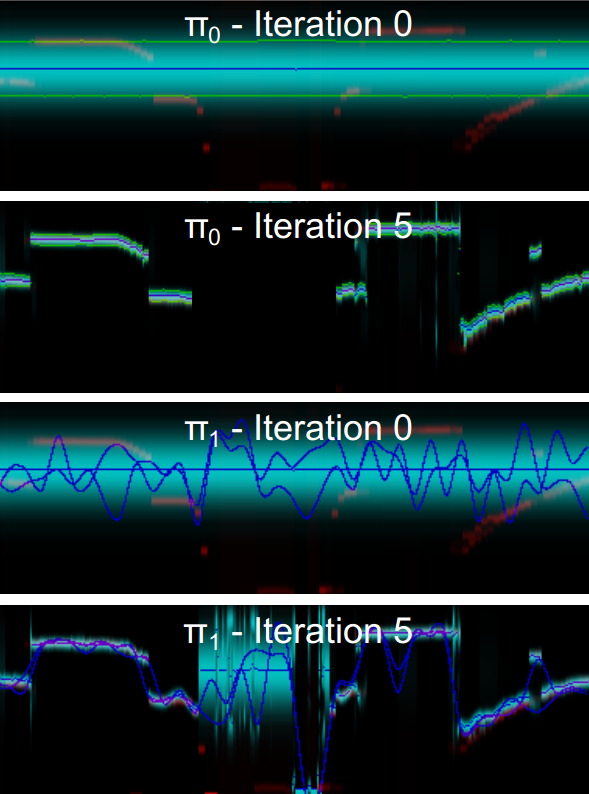
\includegraphics[width=0.49\textwidth]{figures/Uniform.png}
    \end{minipage}\hfill
    \centering
    \caption{\textbf{Left:} Policies $\pi_{0}$ and $\pi_{1}$ where low intensities result in no information (Uniform Distribution). \textbf{Right:} Where low intensities result in an Inverted Gaussian based on our Sensor Model}
    \label{fig:invgau} 
\end{figure}

 \textbf{Effect of Placing more Curtains:} In both policies, placing more light curtains results in much faster convergence, at the cost of increased runtime. Results seen in ~\ref{fig:figure34}

\begin{figure}[h]
    \centering
    \begin{minipage}{0.5\textwidth}
        \centering
        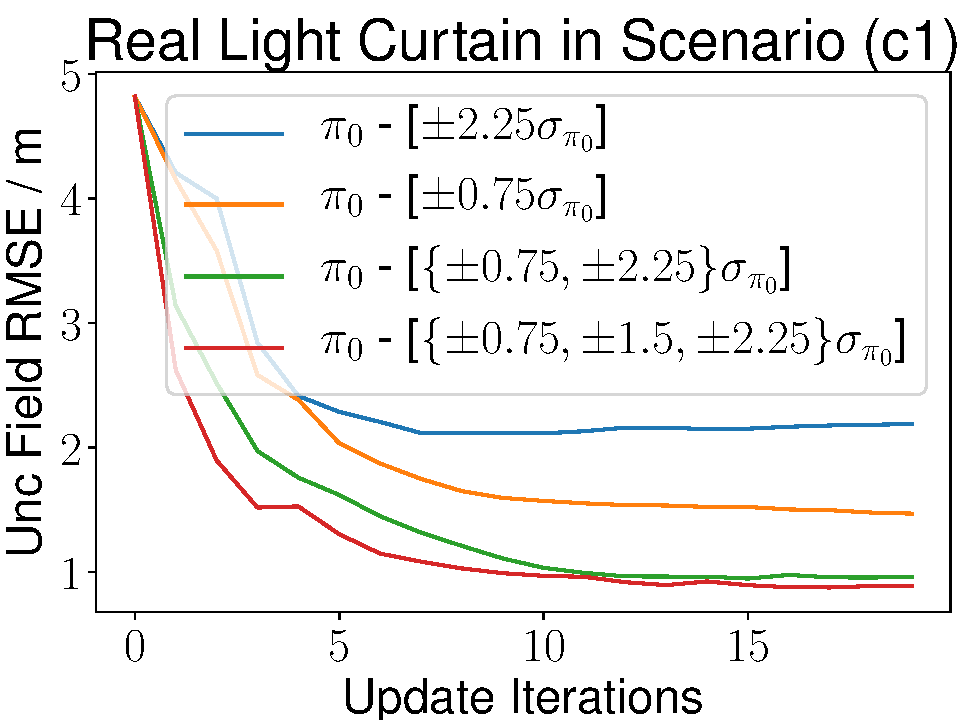
\includegraphics[width=0.49\textwidth]{figures/Figure_3.pdf}
        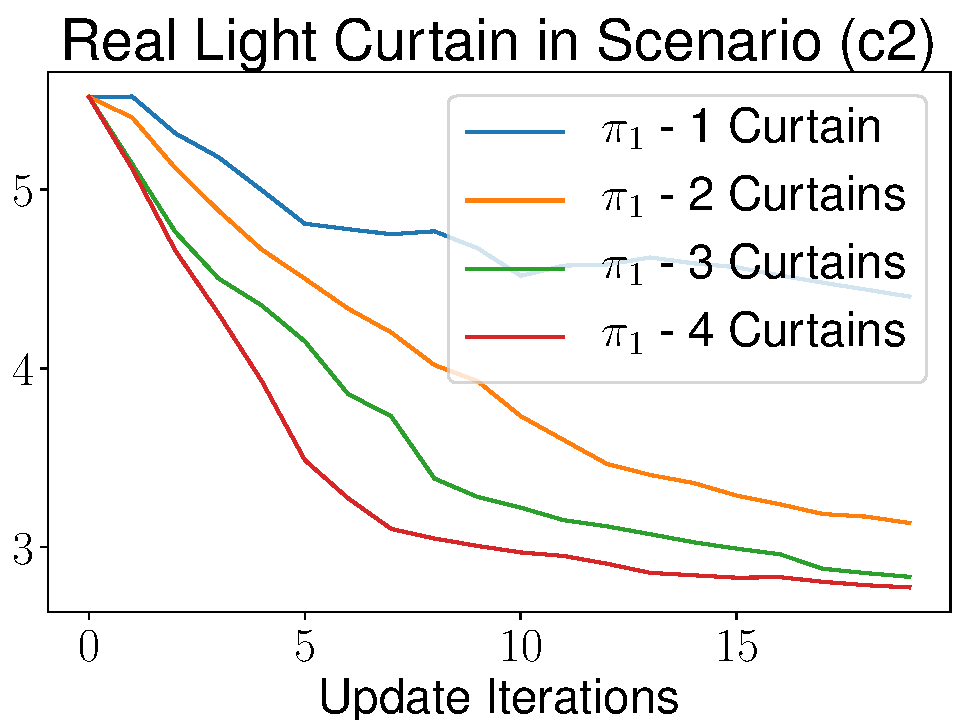
\includegraphics[width=0.49\textwidth]{figures/Figure_4.pdf}
    \end{minipage}\hfill
    \centering
    \caption{Placing more curtains results in faster convergence to the ground truth at the cost of runtime per iteration}
    \label{fig:figure34}
\end{figure}

% While this is a reasonable approach to estimating depth, it is also slow, as it requires placing many curtains. 



{\small
\bibliographystyle{ieee_fullname}
\bibliography{egbib}
}

\end{document}
